\newif\ifteacher\teacherfalse
\documentclass[11pt,a4paper]{article}
\usepackage[margin=2.4cm,top=2.2cm]{geometry}
\usepackage{amsmath,amssymb}
\usepackage{tgschola}\usepackage{fouriernc}
\linespread{1.05}
\usepackage[T1]{fontenc}
\usepackage{microtype}
\usepackage{tikz}
\usetikzlibrary{angles,quotes,calc,arrows.meta}
\usepackage{enumitem}
\usepackage{needspace}
\usepackage{tfrupee}
\definecolor{figline}{RGB}{64,64,64}
\definecolor{figfill}{RGB}{232,232,232}
\definecolor{figfill2}{RGB}{214,214,214}
\definecolor{muted}{RGB}{72,74,78}
\definecolor{thinrule}{RGB}{128,128,128}
\pagestyle{plain}
\setlength{\parindent}{0pt}
\setlength{\parskip}{1pt}
\setlength{\lineskiplimit}{2pt}\setlength{\lineskip}{4pt}
\setlength{\emergencystretch}{2em}
\tikzset{fig/.style={draw=figline}}
\newcommand{\nl}{\\[3pt]}
\newcounter{qn}
\newcommand{\ques}{\par\medskip\refstepcounter{qn}\noindent\hangindent=1.7em\hangafter=1\makebox[1.7em][l]{\textbf{\arabic{qn}.}}\ignorespaces}
\newcommand{\pc}[2]{\par\smallskip\noindent\hspace*{2em}\hangindent=4.3em\hangafter=1\makebox[2em][l]{(#1)}\hspace{0.3em}#2\par}
\newcommand{\mcqone}[4]{\par\smallskip\noindent\hspace*{2em}\hangindent=4.3em\hangafter=1(a)~#1 \qquad (b)~#2 \qquad (c)~#3 \qquad (d)~#4\par}
\newcommand{\mcqtwo}[4]{\par\smallskip\noindent\hspace*{2em}\begin{tabular}[t]{@{}p{0.42\linewidth}@{\hspace{1.6em}}p{0.42\linewidth}@{}}(a)~#1 & (b)~#2 \\[5pt](c)~#3 & (d)~#4\end{tabular}\par\smallskip}
\newcommand{\optline}[1]{\par\vspace{2pt}\noindent\hspace*{2em}\hangindent=4.3em\hangafter=1 #1}
\newcommand{\aritem}[2]{\par\smallskip\noindent\hspace*{1.7em}\hangindent=1.7em\hangafter=1 #1:~#2\par}
\newcommand{\orline}{\par\smallskip{\centering\textit{OR}\par}\nopagebreak\smallskip}
\newcommand{\sect}[1]{\par\medskip\Needspace{15\baselineskip}{\small\bfseries #1}\par\nopagebreak\smallskip}
\ifteacher
\newenvironment{answerblock}
  {\par\needspace{6\baselineskip}\smallskip\begingroup\small\linespread{1.2}\selectfont\color{muted}\noindent\textit{Answer.}\par}
  {\par\endgroup\medskip}
\newcommand{\ap}[1]{\par\smallskip\noindent\textbf{(#1)}\ }
\else
\usepackage{comment}
\excludecomment{answerblock}
\fi
\makeatletter
\newcommand{\figslot}[1]{\@ifundefined{fig@#1}{}{\csname fig@#1\endcsname}}
\makeatother
\makeatletter
\expandafter\def\csname fig@a1\endcsname{%
\begin{center}
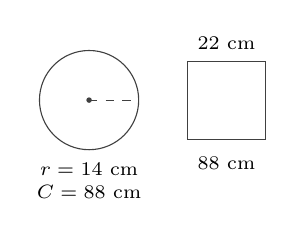
\begin{tikzpicture}[fig,every node/.style={font=\scriptsize}]
\draw[fig] (0,0) circle (0.63);
\fill[figline] (0,0) circle (0.035);
\draw[fig,dashed] (0,0) -- (0.63,0);
\node[below,align=center] at (0,-0.68) {$r=14$~cm\\$C=88$~cm};
\draw[fig] (1.25,-0.495) rectangle (2.24,0.495);
\node[above] at (1.745,0.52) {$22$~cm};
\node[below] at (1.745,-0.6) {$88$~cm};
\end{tikzpicture}
\end{center}}

\expandafter\def\csname fig@a2\endcsname{%
\begin{center}
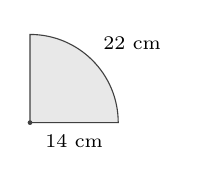
\begin{tikzpicture}[fig,every node/.style={font=\scriptsize}]
\fill[figfill] (0,0) -- (1.12,0) arc (0:90:1.12) -- cycle;
\draw[fig] (0,0) -- (1.12,0) arc (0:90:1.12) -- cycle;
\fill[figline] (0,0) circle (0.03);
\node[below] at (0.56,-0.03) {$14$~cm};
\node[above right] at (45:1.14) {$22$~cm};
\end{tikzpicture}
\end{center}}

\expandafter\def\csname fig@a3\endcsname{%
\begin{center}
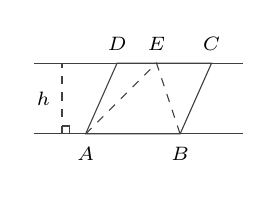
\begin{tikzpicture}[fig,every node/.style={font=\scriptsize}]
\draw[fig,thin] (-0.35,0) -- (2.3,0);
\draw[fig,thin] (-0.35,0.9) -- (2.3,0.9);
\draw[fig] (0.3,0) -- (0.7,0.9) -- (1.9,0.9) -- (1.5,0) -- cycle;
\draw[fig,dashed] (0.3,0) -- (1.2,0.9) -- (1.5,0);
\draw[fig,dashed] (0,0) -- (0,0.9);
\draw[fig] (0,0.1) -- (0.1,0.1) -- (0.1,0);
\node[left] at (-0.03,0.45) {$h$};
\node[below] at (0.3,-0.04) {$A$};
\node[below] at (1.5,-0.04) {$B$};
\node[above] at (0.7,0.94) {$D$};
\node[above] at (1.9,0.94) {$C$};
\node[above] at (1.2,0.94) {$E$};
\end{tikzpicture}
\end{center}}

\expandafter\def\csname fig@a4\endcsname{%
\begin{center}
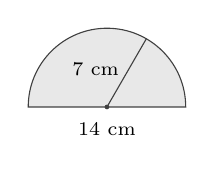
\begin{tikzpicture}[fig,every node/.style={font=\scriptsize}]
\fill[figfill] (-1,0) arc (180:0:1) -- cycle;
\draw[fig] (-1,0) arc (180:0:1) -- cycle;
\fill[figline] (0,0) circle (0.03);
\draw[fig] (0,0) -- (60:1);
\node[left] at (60:0.55) {$7$~cm};
\node[below] at (0,-0.08) {$14$~cm};
\end{tikzpicture}
\end{center}}

\expandafter\def\csname fig@a5\endcsname{%
\begin{center}
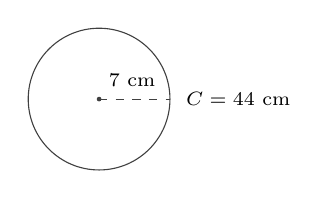
\begin{tikzpicture}[fig,every node/.style={font=\scriptsize}]
\draw[fig] (0,0) circle (0.9);
\fill[figline] (0,0) circle (0.03);
\draw[fig,dashed] (0,0) -- (0.9,0);
\node[above] at (0.42,0.03) {$7$~cm};
\node[right] at (0.98,0) {$C=44$~cm};
\end{tikzpicture}
\end{center}}

\expandafter\def\csname fig@a6\endcsname{%
\begin{center}
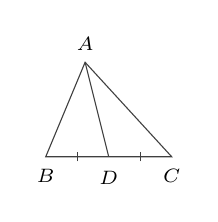
\begin{tikzpicture}[fig,every node/.style={font=\scriptsize}]
\draw[fig] (0,0) -- (1.6,0) -- (0.5,1.2) -- cycle;
\draw[fig] (0.5,1.2) -- (0.8,0);
\draw[fig] (0.4,-0.06) -- (0.4,0.06);
\draw[fig] (1.2,-0.06) -- (1.2,0.06);
\node[above] at (0.5,1.23) {$A$};
\node[below] at (0,-0.04) {$B$};
\node[below] at (1.6,-0.04) {$C$};
\node[below] at (0.8,-0.06) {$D$};
\end{tikzpicture}
\end{center}}

\expandafter\def\csname fig@b7\endcsname{%
\begin{center}
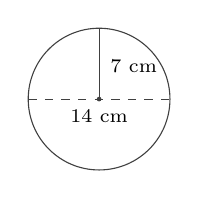
\begin{tikzpicture}[fig,every node/.style={font=\scriptsize}]
\draw[fig] (0,0) circle (0.9);
\fill[figline] (0,0) circle (0.03);
\draw[fig,dashed] (-0.9,0) -- (0.9,0);
\draw[fig] (0,0) -- (0,0.9);
\node[right] at (0.02,0.42) {$7$~cm};
\node[below] at (0,-0.02) {$14$~cm};
\end{tikzpicture}
\end{center}}

\expandafter\def\csname fig@b8\endcsname{%
\begin{center}
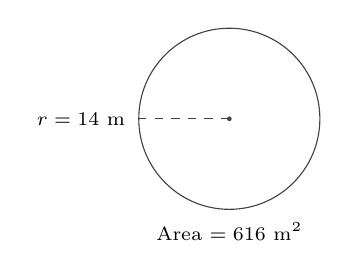
\begin{tikzpicture}[fig,every node/.style={font=\scriptsize}]
\draw[fig] (0,0) circle (1.15);
\fill[figline] (0,0) circle (0.03);
\draw[fig,dashed] (0,0) -- (-1.15,0);
\node[left] at (-1.2,0) {$r=14$~m};
\node[below] at (0,-1.2) {Area $=616$~m$^2$};
\end{tikzpicture}
\end{center}}

\expandafter\def\csname fig@b9\endcsname{%
\begin{center}
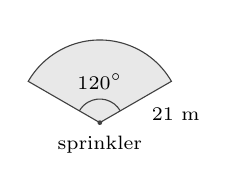
\begin{tikzpicture}[fig,every node/.style={font=\scriptsize}]
\fill[figfill] (0,0) -- (30:1.05) arc (30:150:1.05) -- cycle;
\draw[fig] (0,0) -- (30:1.05) arc (30:150:1.05) -- cycle;
\draw[fig] (30:0.3) arc (30:150:0.3);
\node at (90:0.52) {$120^\circ$};
\node[below right] at (30:0.62) {$21$~m};
\fill[figline] (0,0) circle (0.03);
\node[below] at (0,-0.05) {sprinkler};
\end{tikzpicture}
\end{center}}

\expandafter\def\csname fig@c10\endcsname{%
\begin{center}
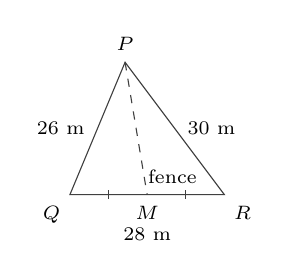
\begin{tikzpicture}[fig,every node/.style={font=\scriptsize}]
\draw[fig] (0,0) -- (1.96,0) -- (0.7,1.68) -- cycle;
\draw[fig,dashed] (0.7,1.68) -- (0.98,0);
\draw[fig] (0.49,-0.055) -- (0.49,0.055);
\draw[fig] (1.47,-0.055) -- (1.47,0.055);
\node[above] at (0.7,1.71) {$P$};
\node[below left] at (0,-0.03) {$Q$};
\node[below right] at (1.96,-0.03) {$R$};
\node[below] at (0.98,-0.03) {$M$};
\node[below] at (0.98,-0.3) {$28$~m};
\node[left] at (0.31,0.84) {$26$~m};
\node[right] at (1.37,0.84) {$30$~m};
\node[right,inner sep=1pt] at (0.95,0.22) {fence};
\end{tikzpicture}
\end{center}}

\expandafter\def\csname fig@c11\endcsname{%
\begin{center}
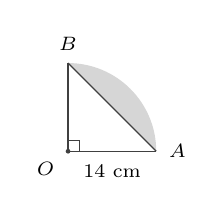
\begin{tikzpicture}[fig,every node/.style={font=\scriptsize}]
\fill[figfill2] (1.12,0) arc (0:90:1.12) -- cycle;
\draw[fig] (0,0) -- (1.12,0);
\draw[fig] (0,0) -- (0,1.12);
\draw[fig] (1.12,0) -- (0,1.12);
\draw[fig] (0.14,0) -- (0.14,0.14) -- (0,0.14);
\fill[figline] (0,0) circle (0.03);
\node[below] at (0.56,-0.05) {$14$~cm};
\node[below left] at (-0.05,-0.02) {$O$};
\node[right] at (1.16,0) {$A$};
\node[above] at (0,1.16) {$B$};
\end{tikzpicture}
\end{center}}

\expandafter\def\csname fig@c12q\endcsname{%
\begin{center}
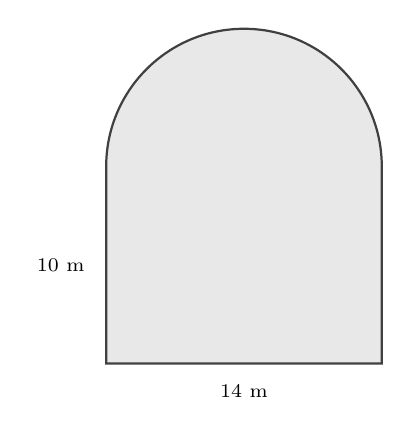
\begin{tikzpicture}[fig,every node/.style={font=\scriptsize}]
\fill[figfill] (-1.75,0) -- (1.75,0) -- (1.75,2.5) arc (0:180:1.75) -- cycle;
\draw[fig,thick] (-1.75,0) -- (1.75,0) -- (1.75,2.5) arc (0:180:1.75) -- cycle;
\node[below] at (0,-0.15) {$14$~m};
\node[left] at (-1.9,1.25) {$10$~m};
\end{tikzpicture}
\end{center}}

\expandafter\def\csname fig@d13\endcsname{%
\begin{center}
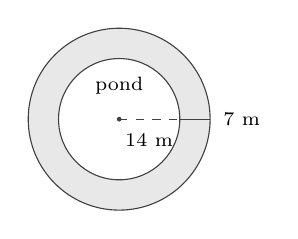
\begin{tikzpicture}[fig,every node/.style={font=\scriptsize}]
\fill[figfill] (0,0) circle (1.155);
\fill[white] (0,0) circle (0.77);
\draw[fig] (0,0) circle (1.155);
\draw[fig] (0,0) circle (0.77);
\draw[fig,dashed] (0,0) -- (0.77,0);
\draw[fig] (0.77,0) -- (1.155,0);
\fill[figline] (0,0) circle (0.03);
\node[below] at (0.38,-0.06) {$14$~m};
\node[right] at (1.2,0) {$7$~m};
\node at (0,0.42) {pond};
\end{tikzpicture}
\end{center}}

\expandafter\def\csname fig@e14q\endcsname{%
\begin{center}
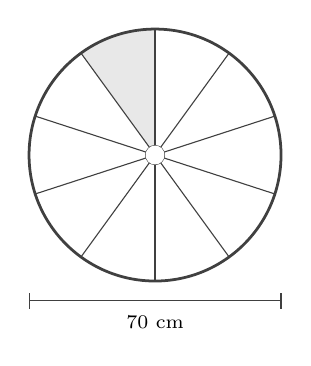
\begin{tikzpicture}[fig,every node/.style={font=\scriptsize}]
\fill[figfill] (0,0) -- (90:1.6) arc (90:126:1.6) -- cycle;
\draw[fig,line width=1pt] (0,0) circle (1.6);
\foreach \a in {18,54,90,126,162,198,234,270,306,342}
  \draw[fig] (\a:0.12) -- (\a:1.6);
\draw[fig] (0,0) circle (0.12);
\fill[white] (0,0) circle (0.12);
\draw[fig] (-1.6,-1.85) -- (1.6,-1.85);
\draw[fig] (-1.6,-1.95) -- (-1.6,-1.75);
\draw[fig] (1.6,-1.95) -- (1.6,-1.75);
\node[below] at (0,-1.92) {$70$~cm};
\end{tikzpicture}
\end{center}}

\expandafter\def\csname fig@e14a\endcsname{%
\begin{center}
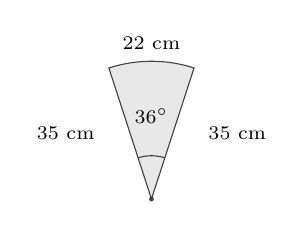
\begin{tikzpicture}[fig,every node/.style={font=\scriptsize}]
\fill[figfill] (0,0) -- (72:1.75) arc (72:108:1.75) -- cycle;
\draw[fig] (0,0) -- (72:1.75) arc (72:108:1.75) -- cycle;
\draw[fig] (72:0.55) arc (72:108:0.55);
\node at (90:1.05) {$36^\circ$};
\node[right] at (0.6,0.83) {$35$~cm};
\node[left] at (-0.6,0.83) {$35$~cm};
\node at (0,1.98) {$22$~cm};
\fill[figline] (0,0) circle (0.03);
\end{tikzpicture}
\end{center}}
\makeatother
\begin{document}
\begin{center}
{\Large\bfseries Perimeter and Area}\\[3pt]
{\large\bfseries Test 3}\\[5pt]
Date: \rule{3cm}{0.4pt} \quad Duration: 1 hour \quad Maximum marks: 30
\end{center}
\vspace{-6pt}
\noindent\rule{\linewidth}{0.6pt}\par
\vspace{3pt}
{\centering\small Use $\pi=\dfrac{22}{7}$. Draw a rough diagram wherever it helps. Show all your steps.\par}
\ifteacher
\vspace{4pt}
{\color{thinrule}\noindent\rule{\linewidth}{0.4pt}}\par
\vspace{4pt}
{\small\color{muted}\linespread{1.15}\selectfont
\textbf{Paper design.} The paper follows the CBSE pattern. Section A: $6\times1$ mark (4 multiple-choice and 2 assertion--reason questions). Section B: $3\times2$ marks. Section C: $3\times3$ marks. Section D: $1\times5$ marks. Section E: 1 case-based question of 4 marks. Total: 30 marks.\nl
\textbf{Competency focus.} Question 9 tests direct application of a formula. The other questions are competency-based. Students compare figures, analyse an error, work backwards from a result, test a claim, or apply results to a real situation.\nl
\textbf{Concepts assessed.} Area and circumference of a circle (Q1, 5, 7, 8, 13, 14); area and perimeter of a sector (Q2, 4, 9, 14); area of a segment (Q11); perimeter and area of a composite figure (Q12); triangles and parallelograms on the same base and between the same parallels (Q3); the median of a triangle (Q6, 10); Heron's formula (Q10).\nl
\textbf{Common misconceptions.} Using the diameter in place of the radius (Q4, 7); leaving out the straight edges from the perimeter of a semicircle or sector (Q4, 12); assuming that figures of equal perimeter have equal areas (Q1); assuming that the area of a ring doubles when its width doubles (Q13).\nl
\textbf{Marking.} Award method marks for a correct set-up, even where the final computation contains an arithmetic error.\par}
\vspace{4pt}
{\color{thinrule}\noindent\rule{\linewidth}{0.4pt}}\par
\vspace{3pt}
\fi

\sect{Section A (1 mark each)}
{\small\itshape Questions 1 to 4 are multiple choice. Questions 5 and 6 are assertion--reason.\par}

\Needspace{7\baselineskip}
\ques A circular rangoli and a square rangoli each have a perimeter of $88$~cm. Which statement is true?\par
\mcqtwo{The circle has the larger area}{The square has the larger area}{The two areas are equal}{The areas cannot be compared without more information}
\begin{answerblock}
\textbf{(a).}\nl
Circle: $2\times\dfrac{22}{7}\times r=88$, so $r=14$~cm. Area $=\dfrac{22}{7}\times14\times14=616$~cm$^2$.\nl
Square: side $=88\div4=22$~cm. Area $=22\times22=484$~cm$^2$.
\figslot{a1}
\end{answerblock}

\Needspace{6\baselineskip}
\ques A sector of a circle has radius $14$~cm. The length of its arc is $22$~cm. What is the area of the sector?\par
\mcqone{$77$~cm$^2$}{$154$~cm$^2$}{$308$~cm$^2$}{$616$~cm$^2$}
\begin{answerblock}
\textbf{(b).}\nl
Circumference $=2\times\dfrac{22}{7}\times14=88$~cm. The arc is $\dfrac{22}{88}=\dfrac14$ of the circumference.\nl
So the sector is $\dfrac14$ of the circle. Area $=\dfrac14\times\dfrac{22}{7}\times14\times14=154$~cm$^2$.
\figslot{a2}
\end{answerblock}

\Needspace{7\baselineskip}
\ques A triangle and a parallelogram stand on the same base and lie between the same parallel lines. The area of the parallelogram is $48$~cm$^2$. What is the area of the triangle?\par
\mcqone{$12$~cm$^2$}{$24$~cm$^2$}{$48$~cm$^2$}{$96$~cm$^2$}
\begin{answerblock}
\textbf{(b).}\nl
The triangle and the parallelogram have the same base and the same height.\nl
Area of the triangle $=\dfrac12\times$ area of the parallelogram $=\dfrac12\times48=24$~cm$^2$.
\figslot{a3}
\end{answerblock}

\Needspace{6\baselineskip}
\ques A protractor is a semicircle of radius $7$~cm. What is the perimeter of the protractor?\par
\mcqone{$22$~cm}{$29$~cm}{$36$~cm}{$44$~cm}
\begin{answerblock}
\textbf{(c).}\nl
Curved edge $=\dfrac12\times2\times\dfrac{22}{7}\times7=22$~cm. Straight edge $=$ diameter $=14$~cm.\nl
Perimeter $=22+14=36$~cm.
\figslot{a4}
\end{answerblock}

\Needspace{13\baselineskip}
\par\medskip\noindent\hangindent=2em\hangafter=0 In Questions 5 and 6, a statement of Assertion (A) is followed by a statement of Reason (R). Choose the correct option.
\optline{(a)~Both A and R are true, and R is the correct explanation of A.}
\optline{(b)~Both A and R are true, but R is not the correct explanation of A.}
\optline{(c)~A is true, but R is false.}
\optline{(d)~A is false, but R is true.}
\par\smallskip

\Needspace{6\baselineskip}
\ques Assertion (A): A circle with circumference $44$~cm has an area of $154$~cm$^2$.\par
\aritem{Reason (R)}{The area of a circle $=\dfrac12\times$ circumference $\times$ radius.}
\begin{answerblock}
\textbf{(a).}\nl
$2\times\dfrac{22}{7}\times r=44$, so $r=7$~cm. Area $=\dfrac12\times44\times7=154$~cm$^2$. A is true.\nl
R is true, because $\pi r^2=\dfrac12\times(2\pi r)\times r$. R gives the method used to obtain A, so R correctly explains A.
\figslot{a5}
\end{answerblock}

\Needspace{6\baselineskip}
\ques Assertion (A): A median of a triangle divides it into two triangles with equal perimeters.\par
\aritem{Reason (R)}{A median of a triangle divides it into two triangles with equal areas.}
\begin{answerblock}
\textbf{(d).}\nl
A is false. The two triangles share the median and have equal halves of the base, but their third sides can differ in length.\nl
R is true. The two triangles have equal bases and the same height.
\figslot{a6}
\end{answerblock}

\sect{Section B (2 marks each)}

\Needspace{8\baselineskip}
\ques A circular cover for a well has a diameter of $14$~cm. Ravi finds its area like this:\par
\vspace{2pt}{\centering Area $=\dfrac{22}{7}\times14\times14=616$~cm$^2$.\par}
\vspace{2pt}\noindent\hspace*{1.7em}Explain Ravi's mistake. Find the correct area of the cover.\par
\begin{answerblock}
Ravi used the diameter, $14$~cm, in place of the radius.\nl
Radius $=14\div2=7$~cm. Area $=\dfrac{22}{7}\times7\times7=154$~cm$^2$.
\figslot{b7}
\end{answerblock}

\Needspace{6\baselineskip}
\ques The area of a circular park is $616$~m$^2$. Find the length of wire needed to fence the park once.\par
\begin{answerblock}
$\dfrac{22}{7}\times r^2=616$, so $r^2=616\times\dfrac{7}{22}=196$ and $r=14$~m.\nl
Length of wire $=$ circumference $=2\times\dfrac{22}{7}\times14=88$~m.
\figslot{b8}
\end{answerblock}

\Needspace{6\baselineskip}
\ques A lawn sprinkler sprays water up to a distance of $21$~m. It turns through an angle of $120^\circ$ and back. Draw a rough diagram. Find the area of the lawn that gets water.\par
\begin{answerblock}
The watered part is a sector of radius $21$~m and angle $120^\circ$.\nl
Area $=\dfrac{120}{360}\times\dfrac{22}{7}\times21\times21=\dfrac13\times1386=462$~m$^2$.
\figslot{b9}
\end{answerblock}

\sect{Section C (3 marks each)}

\Needspace{8\baselineskip}
\ques A triangular plot of land has sides $26$~m, $28$~m and $30$~m.\par
\pc{a}{Find the area of the plot using Heron's formula.}
\pc{b}{The owner wants to divide the plot into two parts of equal area with one straight fence from a corner. Where should the fence meet the opposite side? Give a reason, and find the area of each part.}
\begin{answerblock}
\ap{a} $s=\dfrac{26+28+30}{2}=42$. $s-a=16$, $s-b=14$, $s-c=12$.\nl
Area $=\sqrt{42\times16\times14\times12}=\sqrt{112896}=336$~m$^2$.
\ap{b} The fence must meet the opposite side at its midpoint, so the fence is a median.\nl
A median divides a triangle into two triangles of equal area. Each part $=336\div2=168$~m$^2$.
\figslot{c10}
\end{answerblock}

\Needspace{9\baselineskip}
\ques In a circle with centre $O$ and radius $14$~cm, a chord $AB$ makes an angle of $90^\circ$ at the centre.\par
\pc{a}{Draw a rough diagram. Mark $O$, $A$, $B$, the radius and the angle. Shade the minor segment.}
\pc{b}{Find the area of the minor segment.}
\pc{c}{Find the area of the major segment.}
\begin{answerblock}
\ap{a} See the diagram.
\figslot{c11}
\ap{b} Area of sector $OAB=\dfrac{90}{360}\times\dfrac{22}{7}\times14\times14=154$~cm$^2$.\nl
Area of triangle $OAB=\dfrac12\times14\times14=98$~cm$^2$, since $\angle AOB=90^\circ$.\nl
Minor segment $=154-98=56$~cm$^2$.
\ap{c} Area of the circle $=\dfrac{22}{7}\times14\times14=616$~cm$^2$. Major segment $=616-56=560$~cm$^2$.
\end{answerblock}

\Needspace{16\baselineskip}
\ques A school stage is a rectangle $14$~m long and $10$~m wide, with a semicircle on one of the $14$~m sides, as shown.\par
\nopagebreak
\figslot{c12q}
\pc{a}{A rope is fixed along the whole edge of the stage. Find the length of the rope.}
\pc{b}{Find the area of the stage floor.}
\begin{answerblock}
\ap{a} The semicircle has diameter $14$~m, so its radius is $7$~m.\nl
Curved edge $=\dfrac12\times2\times\dfrac{22}{7}\times7=22$~m. Straight edges $=10+14+10=34$~m.\nl
Rope $=22+34=56$~m.
\ap{b} Rectangle $=14\times10=140$~m$^2$. Semicircle $=\dfrac12\times\dfrac{22}{7}\times7\times7=77$~m$^2$.\nl
Area $=140+77=217$~m$^2$.
\end{answerblock}

\sect{Section D (5 marks)}

\Needspace{12\baselineskip}
\ques A circular pond in a temple garden has a radius of $14$~m. A path $7$~m wide runs around the pond, outside it.\par
\pc{a}{Draw a rough diagram. Find the area of the path. \hfill [2]}
\pc{b}{The path is tiled at \rupee\,$40$ per m$^2$. Find the cost of tiling. \hfill [1]}
\pc{c}{Meena says, ``If the path were $14$~m wide, its area would be double.'' Is Meena right? Show your working and explain. \hfill [2]}
\begin{answerblock}
\ap{a} Outer radius $=14+7=21$~m.\nl
Area of path $=\dfrac{22}{7}\times21\times21-\dfrac{22}{7}\times14\times14=1386-616=770$~m$^2$.
\figslot{d13}
\ap{b} Cost $=770\times40=$ \rupee\,$30800$.
\ap{c} No. Outer radius $=14+14=28$~m.\nl
Area of path $=\dfrac{22}{7}\times28\times28-616=2464-616=1848$~m$^2$.\nl
Double the first path would be $2\times770=1540$~m$^2$. But $1848$~m$^2$ is more than $1540$~m$^2$.\nl
The area of a circle depends on the square of its radius. So the outer part of a wider path adds more area than the inner part.
\end{answerblock}

\sect{Section E (case-based question, 4 marks)}

\Needspace{20\baselineskip}
\ques \textit{Case study: the bicycle wheel.} Lakshmi rides her bicycle to school. Each wheel has a diameter of $70$~cm. Each wheel has $10$ spokes, equally spaced, that run from the centre to the rim.\par
\nopagebreak
\figslot{e14q}
\pc{i}{Find the distance the bicycle moves when the wheel turns once. \hfill [1]}
\pc{ii}{Lakshmi's school is $1.1$~km from her home. How many times does each wheel turn on her way to school? \hfill [1]}
\pc{iii}{Find the area of the part of the wheel between two neighbouring spokes. \hfill [2]}
\orline
\pc{iii}{Find the perimeter of the part of the wheel between two neighbouring spokes. \hfill [2]}
\begin{answerblock}
\ap{i} Radius $=35$~cm. Distance in one turn $=$ circumference $=2\times\dfrac{22}{7}\times35=220$~cm.
\ap{ii} $1.1$~km $=110000$~cm. Number of turns $=110000\div220=500$.
\ap{iii} The $10$ spokes make $10$ equal sectors, each of angle $360^\circ\div10=36^\circ$.\nl
Area of the wheel $=\dfrac{22}{7}\times35\times35=3850$~cm$^2$. Area of one sector $=3850\div10=385$~cm$^2$.
\orline
\ap{iii} Arc of one sector $=220\div10=22$~cm. Perimeter $=22+35+35=92$~cm.
\figslot{e14a}
\end{answerblock}
\end{document}
